%\title{emnlp 2017 instructions}
% File emnlp2017.tex
%

\documentclass[11pt,letterpaper]{article}
\usepackage{emnlp2017}
\usepackage{times}
\usepackage{latexsym}
\usepackage{graphicx}
\usepackage{booktabs}

% Uncomment this line for the final submission:
%\emnlpfinalcopy

%  Enter the EMNLP Paper ID here:
\def\emnlppaperid{***}

% To expand the titlebox for more authors, uncomment
% below and set accordingly.
% \addtolength\titlebox{.5in}    

\newcommand\BibTeX{B{\sc ib}\TeX}


\title{Including lexical morphosyntactic information\\in a neural PoS tagging architecture}

% Author information can be set in various styles:
% For several authors from the same institution:
% \author{Author 1 \and ... \and Author n \\
%         Address line \\ ... \\ Address line}
% if the names do not fit well on one line use
%         Author 1 \\ {\bf Author 2} \\ ... \\ {\bf Author n} \\
% For authors from different institutions:
% \author{Author 1 \\ Address line \\  ... \\ Address line
%         \And  ... \And
%         Author n \\ Address line \\ ... \\ Address line}
% To start a seperate ``row'' of authors use \AND, as in
% \author{Author 1 \\ Address line \\  ... \\ Address line
%         \AND
%         Author 2 \\ Address line \\ ... \\ Address line \And
%         Author 3 \\ Address line \\ ... \\ Address line}
% If the title and author information does not fit in the area allocated,
% place \setlength\titlebox{<new height>} right after
% at the top, where <new height> can be something larger than 2.25in
%\author{Siddharth Patwardhan \and Preethi Raghavan \\
%  {\tt publication@emnlp2017.net}}
\author{Anonymous submission}

\date{}

\begin{document}

\maketitle

\begin{abstract}
  Abstract
\end{abstract}


\section{Introduction}

Part-of-speech tagging is now a classic task in natural language processing, for which many systems have been developed
or adapted for a large variety of languages. Its aim is to associate each ``word'' with a morphosyntactic tag, whose
granularity can range from a simple morphosyntactic category, or part-of-speech (hereafter PoS), to finer categories
enriched with morphological features (gender, number, case, tense, mood, etc.).

The use of machine learning algorithms trained on manually annotated corpora has long become the standard way to develop
PoS taggers. A large variety of algorithms have been used, such as (in approximative chronological order) bigram and
trigram hidden Markov models \cite{merialdo94,brants96,brants00}, decision trees \cite{schmid94,magerman95}, maximum
entropy Markov models (MEMMs) \cite{ratnaparkhi96} and Conditional Random Fields (CRFs)
\cite{lafferty01,constant12}. Recently, neural approaches have reached very competitive accuracy levels, improving over
the state of the art in an number of settings \cite{plank16}.

As a complement to the annotated corpora used to train such systems, external lexical information has been shown to be
valuable sources of information. First, morphosyntactic lexicons, which provide a large inventory of (word,~PoS)
pairs. Such lexical information can be used in the form of constraints at tagging time \cite{kim99,hajic00tagging} or
during the training process as additional features combined with standard features extracted from the training corpus
\cite{chrupala08,goldberg09,denis12}.

Second, lexical information encoded in the form of vector representations, known as word embeddings, have
emerged more recently \cite{bengio03,collobert08,chrupala13,ling15,ballesteros15,muller15}. Such representations, which
are generally extracted from large amounts of raw text, have proved very useful for numerous tasks including PoS
tagging, in particular when used in recurrent neural networks (RNNs) and more specifically in mono- or bi-directional,
word-level and/or character-level long short-term memory networks (LSTMs)
\cite{hochreiter97,ling15,ballesteros15,plank16}.

However, the inclusion of lexical information from morphosyntactic lexicons into neural PoS tagging architecture, as a
replacement or complement to pre-computed word embeddings, remains to be investigated. In this paper, we describe how
such an inclusion can be achieved and show, based on experiments on all corpora from the Universal Dependencies
repository (version 1.3), that it leads to significant improvements over \citeauthor{plank16}'s (\citeyear{plank16}).
state-of-the-art results.

\section{Baseline bi-LSTM tagger}

As shown by \citet{plank16}, state-of-the-art performance can be achieved using a bi-LSTM architecture fed with word
representations. Optimal performance is achieved representing words using the concatenation of (i) a word vector
$\vec{w}$ built using a word embedding layer, called its {\em word embedding}, and (ii) a representation $\vec{c}$ of
the word's characters, called its {\em character-based embedding} built using a character-level bi-LSTM, which is
trained jointly with the word-level layers. Further improvements can be obtained on most but not all languages by
initialising the word embedding layer with pre-computed word embeddings. This baseline architecture is illustrated by
Figure~\ref{fig:schema}(a). We refer to \citet{plank16} for further details.\footnote{In our work, we did not use
  \citeauthor{plank16}'s (\citeyear{plank16}) idea of a secondary task aimed at predicting the frequency class of each
  word. Integrating this secondary task in their bi-LSTM architecture, the authors obtain better OOV scores but
  virtually identical overall scores when averaged over all tested languages/corpora. We therefore decided to stick to
  the standard one-task architecture. }

\section{Integrating lexical morphosyntactic information}

\begin{figure*}
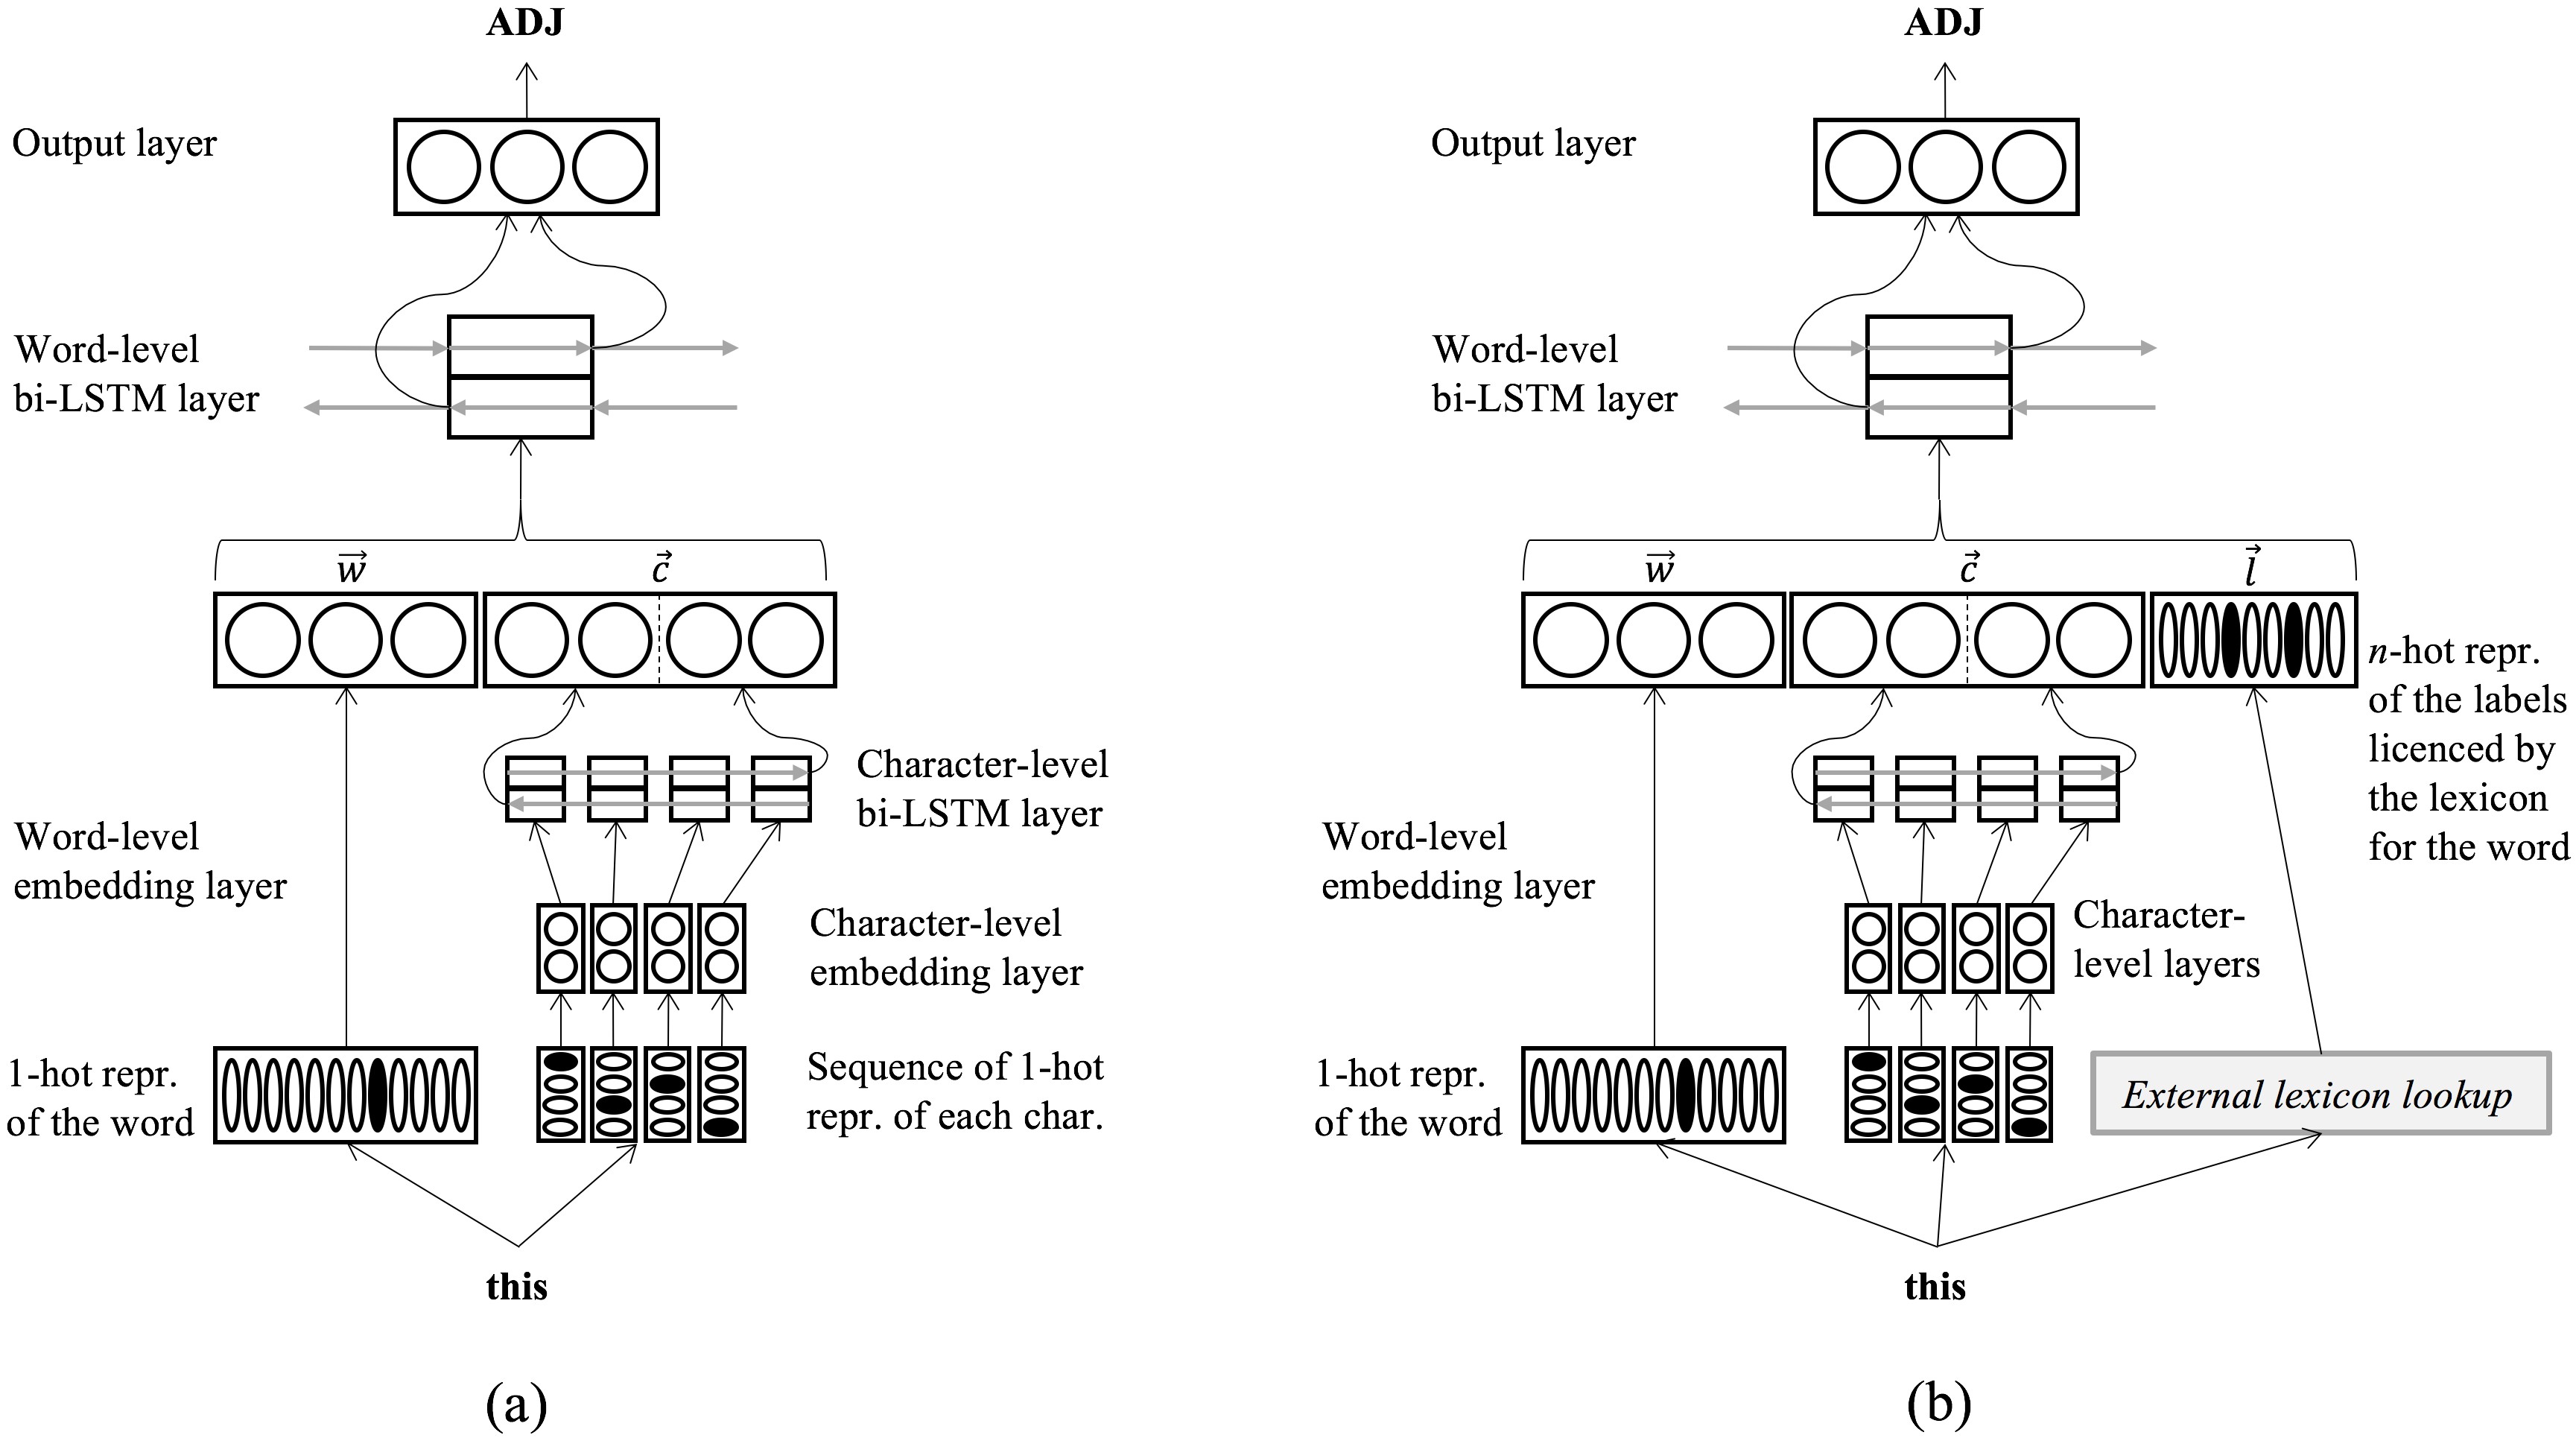
\includegraphics[width=\linewidth]{emnlp17schema}
\caption{Schematic representation of the architecture of (a)~\citeauthor{plank16}'s (\citeyear{plank16}) bi-LSTM tagger,
and (b)~our extension thereof for integrating external morphosyntactic lexical information. Each of these two schemas
represent concern a single word. Connections of the word-level LSTM cells to their counterparts for the preceeding and
following word are represented with grey arrows.}\label{fig:schema}
\end{figure*}

\section{Experiments}

\subsection{Data}

Since the test data of the version 2.0 of the Universal Dependencies corpus collection (hereafter UD) was not available
at the time of the submission, we performed our experiments on a previous version of this corpus collection. More
precisely, in order to facilitate comparison with \citeauthor{plank16}'s (\citeyear{plank16}), we performed all
experiments on the version 1.3 of UD \cite{ud13}.

We used two sets of sources for lexical morphosyntactic information, which we will refer to respectively as {\sc lex}
and {\sc lex2}. Quantitative information about these lexicons is provided in Table~\ref{tbl:lex}.

The {\sc lex} series of lexicons have been extracted from freely available morphological lexicons or analysers developed
for the Apertium\footnote{\url{https://svn.code.sf.net/p/apertium/svn/languages}} and the
Giellatekno\footnote{\url{https://victorio.uit.no/langtech/trunk/langs}} projects. For languages for which an Apertium
morphological lexicon is available, this lexicon was used. For other languages, we downloaded from the OPUS corpus
collection the corresponding monolingual part of OpenSubtitles2016, tokenised it, extracted the 1 million most frequent
tokens, and retrieved all their morphological analyser by the Apertium morphological transducer ---or by the Giellatekno
morphological transducer when none was available from Apertium. All these analyses were then gathered in the form of a
lexicon. In a second step, we converted all lexicons obtained using manually crafted rules, so that each lexical entry
contains a (inflected) wordform, a lemma, a PoS from the Universal POS
tagset,\footnote{\url{http://universaldependencies.org/u/pos/all.html}} and a set of attribute-value pairs from the
Universal Features.\footnote{\url{http://universaldependencies.org/u/feat/all.html}} In Table~\ref{tbl:lex}, lexicons
directly converted from Apertium lexicons have type {\em ap.lex}, lexicons obtained via Apertium morphological analysers
have type {\em ap.ma}, and lexicons obtained via Giellatekno morphological analysers
have type {\em ap.gt}.

The {\sc lex2} series of lexicons have been gather from numerous sources. For space reasons, we are not able to describe
here the language-specific transformations we applied to some of these lexicons. References are given in
Table~\ref{tbl:lex}.

Finally, whenever available and following \citet{plank16}, we performed experiments using Polyglot pre-computed
embeddings published by \citet{alrfou13}. Languages for which Polyglot embeddings are available are indicated in Table~\ref{tbl:lex}.

\begin{table*}
\centering
\scriptsize
\begin{tabular}{l|lrr|llrrc}
\toprule
Lang. & \multicolumn{3}{c}{\sc lex} & \multicolumn{3}{|c}{\sc lex2} & Polyglot\\
code & type & \#entries & \#tags (full/coarse) & name & reference & \#entries & \#tags & embeds\\
\midrule
ar & {\em ap.lex} & 650592 & 658/15 &  &  &  &  & yes\\
bg & {\em ap.lex} & 93186 & 286/16 & MULTEXT-East V4 & \citep{erjavec10} & 53056 & 12 & yes\\
ca & {\em ap.lex} & 369927 & 188/13 &  &  &  &  & yes\\
cs & {\em ap.lex} & 1874737 & 1119/15 & Morfflex (filtered) & \citep{hajic13} & 2094860 & 65 & yes\\
da & {\em ap.lex} & 683456 & 164/15 & STO & \citep{braasch08} & 591035 & 45 & yes\\
de & {\em ap.lex} & 2179689 & 536/16 & DeLex & \citep{sagot14delex} & 465434 & 52 & yes\\
el & {\em ap.lex} & 47131 & 190/12 & DELA\_gr & \citep{symeonidis99} & 1988898 & 25 & yes\\
en & {\em ap.lex} & 126928 & 108/15 & EnLex & \citep{sagot10lefff} & 490511 & 47 & yes\\
es & {\em ap.lex} & 324517 & 157/12 & Le{\it ff}e & \citep{molinero09} & 755858 & 34 & yes\\
et & {\em gt.ma} & 43553 & 202/12 & MULTEXT-East V4 & \citep{erjavec10} & 133804 & 11 & yes\\
eu & {\em ap.lex} & 52618 & 37/14 &  &  &  &  & yes\\
fa &  &  &  & PerLex & \citep{sagot10perlex} & 511840 & 37 & yes\\
fi & {\em gt.ma} & 227530 & 202/13 &  &  &  &  & yes\\
fr & {\em ap.lex} & 136025 & 135/13 & Le{\it fff} & \citep{sagot10lefff} & 539278 & 25 & yes\\
ga &  &  &  & inmdb & \citep{mechura14} & 113975 & 32 & yes\\
gl & {\em ap.lex} & 240698 & 165/13 & LeffGa & \citep{sagot10lefff} & 742954 & 28 & \\
grc &  &  &  & Diogenes (Greek) & \citep{heslin07} & 3911616 & 14531 & \\
he & {\em ap.lex} & 267533 & 107/16 &  &  &  &  & yes\\
hi & {\em ap.lex} & 158605 & 201/14 &  &  &  &  & yes\\
hr &  &  &  & HML & \citep{oliver04} & 1360687 & 22 & yes\\
hu & {\em gt.ma} & 2937 & 4/3 & MULTEXT-East V4 & \citep{erjavec10} & 75354 & 834 & \\
id & {\em ap.lex} & 12199 & 38/14 & Kateglo & \scalebox{0.9}{\url{github.com/ivanlanin/kateglo}} & 72217 & 118 & yes\\
it & {\em ap.lex} & 278356 & 154/14 & Morph it! & \citep{zanchetta05} & 422756 & 16 & yes\\
kk & {\em gt.ma} & 434119 & 1274/16 &  &  &  &  & \\
la &  &  &  & Diogenes (Latin) & \citep{heslin07} & 1231619 & 872 & \\
lv & {\em ap.lex} & 313642 & 583/14 &  &  &  &  & \\
nl & {\em ap.lex} & 167302 & 85/14 & Alpino lexicon V1 & \citep{bouma00} & 80928 & 65 & yes\\
no & {\em ap.lex} & 2469905 & 158/13 & OrdBank & \citep{hagen10} & 880503 & 224 & yes\\
pl & {\em ap.lex} & 1316112 & 1592/15 & PolLex & \citep{sagot07ltc} & 1399697 & 1082 & yes\\
pt & {\em ap.lex} & 158504 & 155/14 & Labellex\_pt & \citep{ranchhod99} & 1258205 & 281 & yes\\
ro & {\em ap.lex} & 229341 & 247/13 & MULTEXT-East V4 & \citep{erjavec10} & 378113 & 14 & \\
ru & {\em ap.lex} & 4400935 & 847/16 &  &  &  &  & \\
sl & {\em ap.lex} & 653965 & 1110/14 & SloLeks & \citep{krek08} & 957525 & 25 & yes\\
sv & {\em ap.lex} & 2378232 & 205/12 & Saldo & \citep{borin08} & 1214971 & 214 & yes\\
tr & {\em gt.ma} & 417340 & 1764/14 &  &  &  &  & \\
zh & {\em ap.lex} & 7617 & 14/13 &  &  &  &  & \\
\bottomrule
\end{tabular}
\caption{Information about lexical informations used in this paper.}\label{tbl:lex}
\end{table*}

\subsection{Experimental setup}

We use as a baseline the state-of-the-art bi-LSTM PoS tagger \texttt{bilty}, a freely
available\footnote{\url{https://github.com/bplank/bilstm-aux}} and ``significantly refactored version of the code
originally used in'' \cite{plank16}. We use its standard configuration, with only one bi-LSTM layer.

We extended \texttt{bilty} for enabling integration of lexical morphosyntactic information, in the way described in the
previous section.\footnote{We also performed alternative experiments in which the word-to-set-of-lexical-labels mapping
  was not fixed, but was initialised using the lexical information and then updated in the same way as a standard
  embedding layer. This resulted in slightly better accuracy scores, but also in a massively increased memory
  usage. Because such a setting is therefore not tractable in practice for most language and most users, we decided to
  stick to a fixed word-to-set-of-lexical-labels mapping.}

For each lexicon-related configuration, we trained three variants of the tagger: (i)~a variant without using
character-based embeddings and standard (zero) initialisation of word embeddings before training, (ii)~a variant with
character-based embeddings and standard initialisation of word embeddings, and (iii)~when Polyglot embeddings are
available for the language at hand, a variant with character-based embeddings and initialisation of the word embeddings
with the Polyglot embeddings. This is deliberately similar to \citeauthor{plank16}'s (\citeyear{plank16}) experimental
setup, in order to facilitate the comparison of results.

Note that we discarded alternative UD 1.3 corpora (e.g., {\tt nl\_lassysmall} as opposed to {\tt nl}), as well as
corpora for languages for which we had neither a lexicon nor Polyglot embeddings (Old Church Slavonic, Gothic and Tamil).


\section{Results and discussion}


%\section*{Acknowledgments}



\bibliography{emnlp17}
\bibliographystyle{emnlp_natbib}

\end{document}
